
\documentclass[border=10pt, 12pt]{standalone}
\usepackage[svgnames]{xcolor}
\usepackage{amsmath}
\usepackage{pgfplots}
\pgfplotsset{compat=newest}
\usepackage[sfdefault]{FiraSans}
\usepackage{FiraMono}
\renewcommand*\familydefault{\sfdefault}
\begin{document}
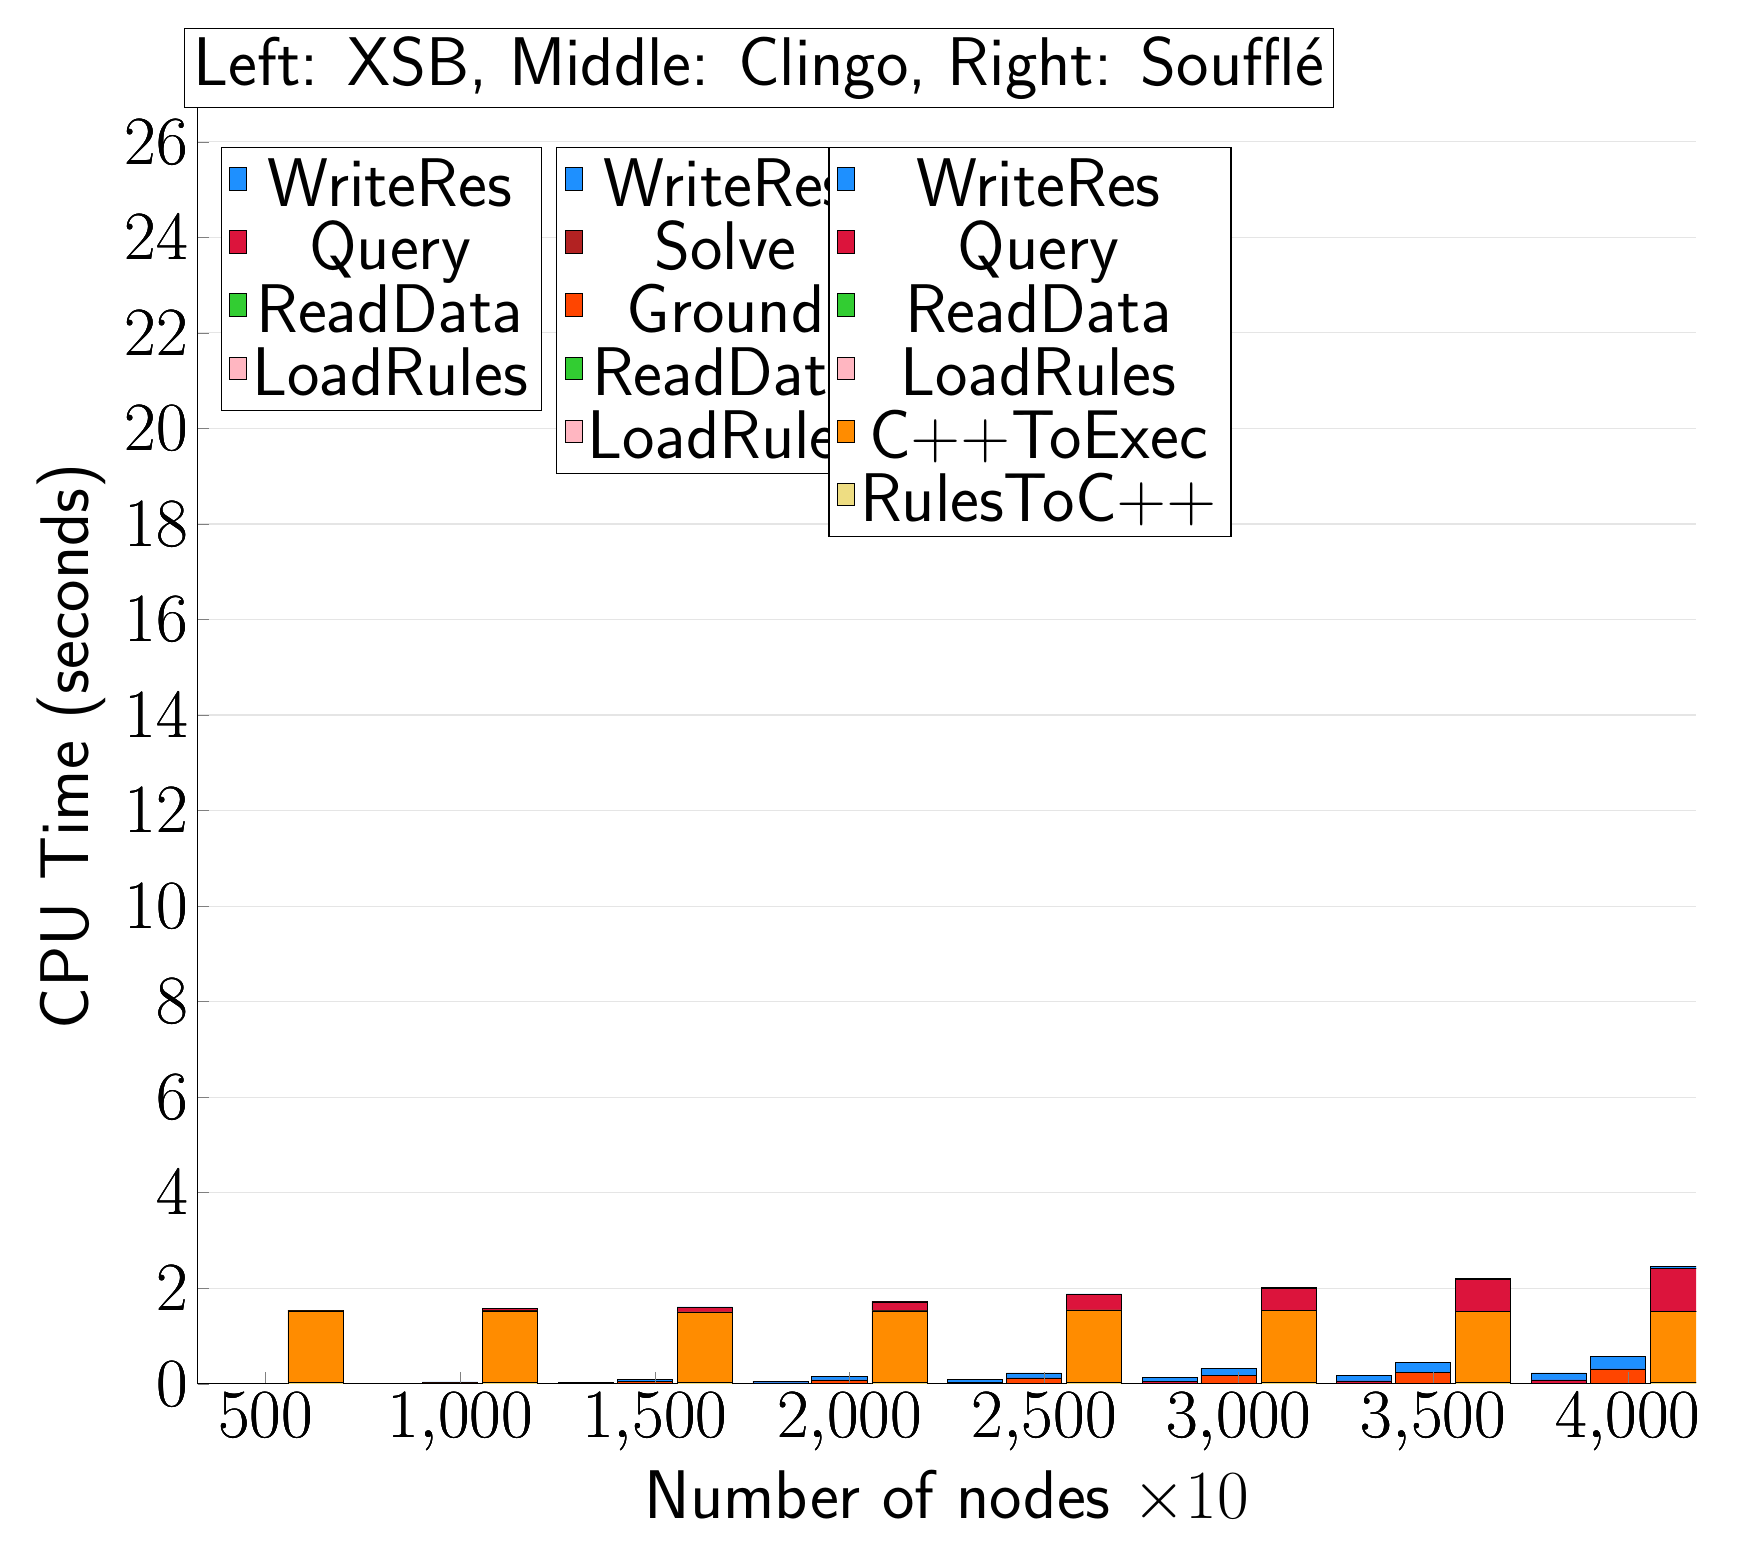
\begin{tikzpicture}
	\begin{axis}[bar shift=-25pt,
			ybar stacked,
			width=1.7\textwidth,
			bar width=0.7cm,
			ymajorgrids, tick align=inside,
			major grid style={draw=gray!20},
			xtick=data,
			ymin=0, ymax=26.698890000000002,
			axis x line*=bottom,
			axis y line*=left,
			enlarge x limits=0.05,
			legend style={
					at={(0.23, 0.97)},
					anchor=north east,
					legend columns=1,
					font=\Huge,
				},
			ylabel={CPU Time (seconds)},
			xlabel={Number of nodes $\times 10$},
			label style={font=\Huge},
			tick label style={font=\Huge},
		]
		\addlegendimage{fill=DodgerBlue, draw=black, line width=0.2pt}
		\addlegendentry{WriteRes}
		\addlegendimage{fill=Crimson, draw=black, line width=0.2pt}
		\addlegendentry{Query}
		\addlegendimage{fill=LimeGreen, draw=black, line width=0.2pt}
		\addlegendentry{ReadData}
		\addlegendimage{fill=LightPink, draw=black, line width=0.2pt}
		\addlegendentry{LoadRules}
		\addplot +[fill=LightPink, draw=black, line width=0.2pt] coordinates {
				(500, 0.0006163999999999998)
				(1000, 0.0006118)
				(1500, 0.0006055000000000004)
				(2000, 0.0006146000000000004)
				(2500, 0.0006238000000000001)
				(3000, 0.0006349999999999996)
				(3500, 0.0006086999999999993)
				(4000, 0.0006159999999999997)
			};
		\addplot +[fill=LimeGreen, draw=black, line width=0.2pt] coordinates {
				(500, 0.0005880000000000002)
				(1000, 0.0010717)
				(1500, 0.0015432)
				(2000, 0.002051)
				(2500, 0.0025302000000000002)
				(3000, 0.0030497)
				(3500, 0.0034939999999999997)
				(4000, 0.0040036)
			};
		\addplot +[fill=Crimson, draw=black, line width=0.2pt] coordinates {
				(500, 0.0011064)
				(1000, 0.0045603)
				(1500, 0.010622900000000001)
				(2000, 0.0188502)
				(2500, 0.0291761)
				(3000, 0.0431721)
				(3500, 0.057005099999999996)
				(4000, 0.0783614)
			};
		\addplot +[fill=DodgerBlue, draw=black, line width=0.2pt] coordinates {
				(500, 0.0022721000000000004)
				(1000, 0.0093611)
				(1500, 0.0209868)
				(2000, 0.0367775)
				(2500, 0.0568887)
				(3000, 0.0822341)
				(3500, 0.11212)
				(4000, 0.14634699999999998)
			};
	\end{axis}

	\begin{axis}[bar shift=-3.7pt,
			ybar stacked,
			width=1.7\textwidth,
			bar width=0.7cm,
			ymajorgrids, tick align=inside,
			major grid style={draw=none},
			xtick=data,
			ymin=0, ymax=26.698890000000002,
			axis x line*=none,
			axis y line*=none,
			enlarge x limits=0.05,
			legend style={
					at={(0.454, 0.97)},
					anchor=north east,
					legend columns=1,
					font=\Huge,
				},
			label style={font=\Huge},
			tick label style={font=\Huge},
		]
		\addlegendimage{fill=DodgerBlue, draw=black, line width=0.2pt}
		\addlegendentry{WriteRes}
		\addlegendimage{fill=FireBrick, draw=black, line width=0.2pt}
		\addlegendentry{Solve}
		\addlegendimage{fill=OrangeRed, draw=black, line width=0.2pt}
		\addlegendentry{Ground}
		\addlegendimage{fill=LimeGreen, draw=black, line width=0.2pt}
		\addlegendentry{ReadData}
		\addlegendimage{fill=LightPink, draw=black, line width=0.2pt}
		\addlegendentry{LoadRules}
		\addplot +[fill=LightPink, draw=black, line width=0.2pt] coordinates {
				(500, 0.0)
				(1000, 0.0)
				(1500, 0.0)
				(2000, 0.0)
				(2500, 0.0)
				(3000, 0.0)
				(3500, 0.0)
				(4000, 0.0)
			};
		\addplot +[fill=LimeGreen, draw=black, line width=0.2pt] coordinates {
				(500, 0.0)
				(1000, 0.0)
				(1500, 0.005999999999999998)
				(2000, 0.009999999999999997)
				(2500, 0.008999999999999998)
				(3000, 0.009999999999999998)
				(3500, 0.009999999999999997)
				(4000, 0.009999999999999997)
			};
		\addplot +[fill=OrangeRed, draw=black, line width=0.2pt] coordinates {
				(500, 0.009999999999999997)
				(1000, 0.019999999999999997)
				(1500, 0.04400000000000001)
				(2000, 0.07000000000000002)
				(2500, 0.11200000000000002)
				(3000, 0.16199999999999998)
				(3500, 0.22400000000000003)
				(4000, 0.28900000000000003)
			};
		\addplot +[fill=FireBrick, draw=black, line width=0.2pt] coordinates {
				(500, 0.0)
				(1000, 0.0)
				(1500, 0.0)
				(2000, 0.0)
				(2500, 0.001999999999999996)
				(3000, 0.004000000000000001)
				(3500, 0.01100000000000001)
				(4000, 0.014000000000000012)
			};
		\addplot +[fill=DodgerBlue, draw=black, line width=0.2pt] coordinates {
				(500, 0.0)
				(1000, 0.019999999999999993)
				(1500, 0.038999999999999986)
				(2000, 0.07000000000000002)
				(2500, 0.10400000000000001)
				(3000, 0.14699999999999996)
				(3500, 0.19999999999999998)
				(4000, 0.26199999999999996)
			};
	\end{axis}

	\begin{axis}[bar shift=18pt,
			ybar stacked,
			width=1.7\textwidth,
			bar width=0.7cm,
			ymajorgrids, tick align=inside,
			major grid style={draw=none},
			xtick=data,
			ymin=0, ymax=26.698890000000002,
			axis x line*=none,
			axis y line*=none,
			enlarge x limits=0.05,
			legend style={
					at={(0.69, 0.97)},
					anchor=north east,
					legend columns=1,
					font=\Huge,
				},
			label style={font=\Huge},
			tick label style={font=\Huge},
		]
		\addlegendimage{fill=DodgerBlue, draw=black, line width=0.2pt}
		\addlegendentry{WriteRes}
		\addlegendimage{fill=Crimson, draw=black, line width=0.2pt}
		\addlegendentry{Query}
		\addlegendimage{fill=LimeGreen, draw=black, line width=0.2pt}
		\addlegendentry{ReadData}
		\addlegendimage{fill=LightPink, draw=black, line width=0.2pt}
		\addlegendentry{LoadRules}
		\addlegendimage{fill=DarkOrange, draw=black, line width=0.2pt}
		\addlegendentry{C++ToExec}
		\addlegendimage{fill=LightGoldenrod, draw=black, line width=0.2pt}
		\addlegendentry{RulesToC++}
		\addplot +[fill=LightGoldenrod, draw=black, line width=0.2pt] coordinates {
				(500, 0.030000000000000006)
				(1000, 0.030000000000000006)
				(1500, 0.030000000000000006)
				(2000, 0.030000000000000006)
				(2500, 0.030000000000000006)
				(3000, 0.030000000000000006)
				(3500, 0.030000000000000006)
				(4000, 0.030000000000000006)
			};
		\addplot +[fill=DarkOrange, draw=black, line width=0.2pt] coordinates {
				(500, 1.499)
				(1000, 1.499)
				(1500, 1.4700000000000002)
				(2000, 1.498)
				(2500, 1.5110000000000001)
				(3000, 1.502)
				(3500, 1.479)
				(4000, 1.482)
			};
		\addplot +[fill=LightPink, draw=black, line width=0.2pt] coordinates {
				(500, 9.549999999999999e-05)
				(1000, 0.0001109)
				(1500, 7.55e-05)
				(2000, 9.52e-05)
				(2500, 7.819999999999999e-05)
				(3000, 0.00010410000000000001)
				(3500, 0.0001227)
				(4000, 0.000108)
			};
		\addplot +[fill=LimeGreen, draw=black, line width=0.2pt] coordinates {
				(500, 0.0013733)
				(1000, 0.0026395)
				(1500, 0.0037284000000000006)
				(2000, 0.0047845)
				(2500, 0.0054067)
				(3000, 0.0070896)
				(3500, 0.0088945)
				(4000, 0.0098764)
			};
		\addplot +[fill=Crimson, draw=black, line width=0.2pt] coordinates {
				(500, 0.012786199999999998)
				(1000, 0.044885800000000003)
				(1500, 0.1024462)
				(2000, 0.1844246)
				(2500, 0.31751310000000005)
				(3000, 0.46051449999999994)
				(3500, 0.6629084000000001)
				(4000, 0.8883324)
			};
		\addplot +[fill=DodgerBlue, draw=black, line width=0.2pt] coordinates {
				(500, 0.0011163999999999998)
				(1000, 0.0029163)
				(1500, 0.0063707)
				(2000, 0.0113031)
				(2500, 0.017820500000000003)
				(3000, 0.025337600000000005)
				(3500, 0.034159100000000005)
				(4000, 0.0449107)
			};
	\end{axis}


	\node[anchor=south, draw, fill=white] at (rel axis cs:0.42,1) {\Huge Left: XSB, Middle: Clingo, Right: Soufflé};
\end{tikzpicture}
\end{document}
